
\q{30}{CSPs}
\begin{question}[]{\bf Pacman's new house}

After years of struggling through mazes, Pacman has finally made peace with the ghosts, Blinky, Pinky, Inky, and Clyde, and invited them to live with him and Ms. Pacman. The move has forced Pacman to change the rooming assignments in his house, which has 6 rooms. He has decided to figure out the new assignments with a CSP in which the variables are Pacman \textbf{(P)}, Ms. Pacman \textbf{(M)}, Blinky \textbf{(B)}, Pinky \textbf{(K)}, Inky \textbf{(I)}, and Clyde \textbf{(C)}, the values are which room they will stay in, from 1-6, and the constraints are:
\begin{table}[h]
\centering
\begin{tabular}{ll}
i) No two agents can stay in the same room&\\
ii) \textbf{P} $>$ 3 &
vi) \textbf{B} is even\\
iii) \textbf{K} is less than \textbf{P}&
vii) \textbf{I} is not 1 or 6\\
iv) \textbf{M} is either 5 or 6&
viii) $\vert$\textbf{I}-\textbf{C}$\vert$ = 1\\
v) \textbf{P} $>$ \textbf{M}&
ix) $\vert$\textbf{P}-\textbf{B}$\vert$ = 2
\end{tabular}
\end{table}
\begin{subquestion}[1]{\bf Unary constraints}
On the grid below cross out the values from each domain that are eliminated by enforcing unary constraints.
\solution{
\begin{table}[h]
\centering
\begin{tabular}{ccccccc}
P & 1 & 2 & 3 & 4 & 5 & 6\\
B & 1 & 2 & 3 & 4 & 5 & 6\\
C & 1 & 2 & 3 & 4 & 5 & 6\\
K & 1 & 2 & 3 & 4 & 5 & 6\\
I & 1 & 2 & 3 & 4 & 5 & 6\\
M & 1 & 2 & 3 & 4 & 5 & 6\\
\end{tabular}
\end{table}
}{
\begin{table}[h]
\centering
\begin{tabular}{ccccccc}
\AnswerOneAi
\end{tabular}
\end{table}
}
\end{subquestion}
\begin{subquestion}[1]{\bf MRV}
According to the Minimum Remaining Value (MRV) heuristic, which variable should be assigned to first?\\\\
\AnswerOneAii

\end{subquestion}

\begin{subquestion}[3]{\bf Forward Checking}
For the purposes of decoupling this problem from your solution to the
previous problem, assume we choose to assign P first, and assign it the value 6. What are the resulting domains after enforcing unary constraints (from part i) and running forward checking for this assignment?
\solution{
\begin{table}[h]
\centering
\begin{tabular}{ccccccc}
P &   &   &   &  &   &  6\\
B & 1 & 2 & 3 & 4 & 5 & 6\\
C & 1 & 2 & 3 & 4 & 5 & 6\\
K & 1 & 2 & 3 & 4 & 5 & 6\\
I & 1 & 2 & 3 & 4 & 5 & 6\\
M & 1 & 2 & 3 & 4 & 5 & 6\\

\end{tabular}
\end{table}
}{
\begin{table}[h]
\begin{center}
\begin{tabular}{ccccccc}
\AnswerOneAiii
\end{tabular}
\end{center}
\end{table}

}
\end{subquestion}

\begin{subquestion}[3]{\bf Iterative Improvement}
Instead of running backtracking search, you decide to start over and run
iterative improvement with the min-conflicts heuristic for value selection. Starting with the following assignment:\\\\
P:6, B:4, C:3, K:2, I:1, M:5\\\\
First, for each variable write down how many constraints it violates in the table below.\\
Then, in the table on the right, for all variables that could be selected for assignment, put an x in any box that corresponds to a possible value that could be assigned to that variable according to min-conflicts \textbf{in the next iteration}. When marking next values a variable could take on, only mark values different from the current one.

\begin{center}
\begin{tabular}{cc}
\begin{tabular}{|c|c|}
\hline
\AnswerOneAiv
\end{tabular}
\end{tabular}
\end{center}
\end{subquestion}

\end{question}
\newpage
\begin{question}[]{\bf Variable ordering}\\
We say that a variable X is backtracked if, after a value has been assigned to X, the recursion returns at X without a solution, and a different value must be assigned to X.\\
For this problem, consider the following three algorithms:
\begin{enumerate}
\item
Run backtracking search with no filtering
\item 
Initially enforce arc consistency, then run backtracking search with no filtering
\item
Initially enforce arc consistency, then run backtracking search while enforcing arc consistency after each assignment\\
\end{enumerate}

\begin{subquestion}[6]{}\\
For each algorithm, circle all orderings of variable assignments that guarantee that no backtracking will be necessary when finding a solution to the CSP represented by the following constraint graph.\\\\
\begin{table}[h]
\begin{tabular}{cc}
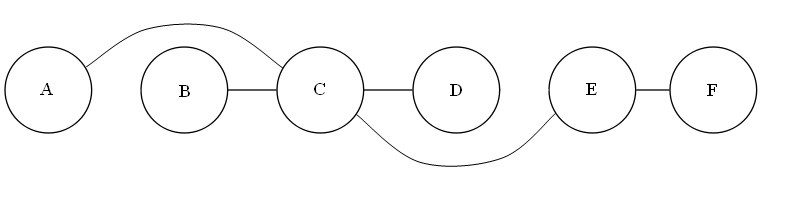
\includegraphics[scale=.4]{figures/tree.png}
&
\begin{tabular}{c|c|c}
\AnswerOneBi
\end{tabular}
\end{tabular}
\end{table}\\

\end{subquestion}
\begin{subquestion}[6]{}\\
For each algorithm, circle all orderings of variable assignments that guarantee that no more than two variables will be backtracked when finding a solution to the CSP represented by the following constraint graph.\\\\

\begin{table}[h]
\centering
\begin{tabular}{cc}
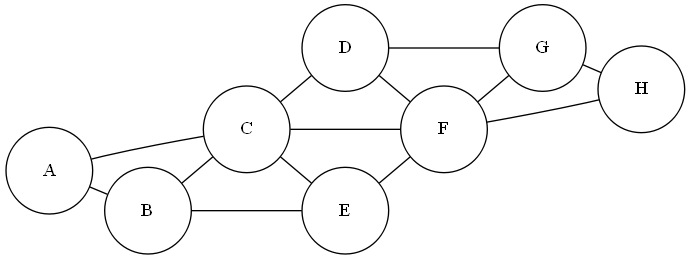
\includegraphics[scale=.3]{figures/csp_graph.png}
&
\begin{tabular}{c|c|c}
\AnswerOneBii
\end{tabular}
\end{tabular}
\end{table}
\end{subquestion}
\end{question}
\newpage
\begin{question}[]{\bf All Satisfying Assignments}
Now consider a modified CSP in which we wish to find every possible satisfying assignment, rather than just one such assignment as in normal CSPs. In order to solve this new problem, consider a new algorithm which is the same as the normal backtracking search algorithm, except that when it sees a solution, instead of returning it, the solution gets added to a list, and the algorithm backtracks. Once there are no variables remaining to backtrack on, the algorithm returns the list of solutions it has found.\\\\
For each graph below, select whether or not using the MRV and/or LCV heuristics could affect the number of leaf nodes in the search tree in this new situation.


\begin{subquestion}[2]{}\\
\begin{tabular}{cl}
\multirow{1}{*}{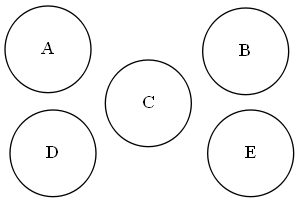
\includegraphics[scale=0.5]{figures/disconnected.png} \hspace{1.4in}}
\AnswerOneCi

\end{tabular}\\
\end{subquestion}

\vspace{-.1in}
\begin{subquestion}[2]{}\\
\begin{tabular}{cl}


\multirow{1}{*}{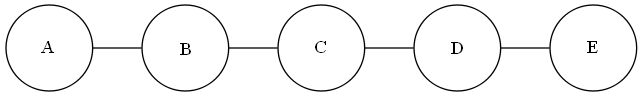
\includegraphics[scale=0.5]{figures/chain.png} \hspace{0.260in}}
\AnswerOneCii

\end{tabular}\\
\end{subquestion}
\vspace{-.19in}
\begin{subquestion}[2]{}\\
\begin{tabular}{cl}

\multirow{1}{*}{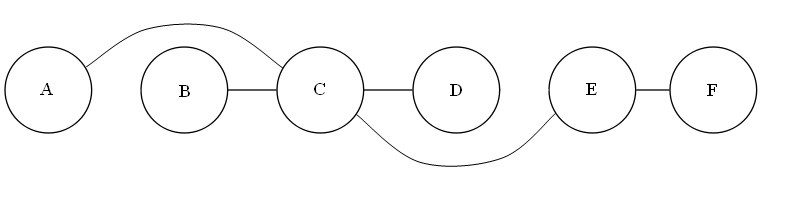
\includegraphics[width=3in]{figures/tree.png}}\\\\
\AnswerOneCiii

\end{tabular}
\end{subquestion}
\vspace{-.19in}
\begin{subquestion}[2]{}\\
\begin{tabular}{cl}

\multirow{1}{*}{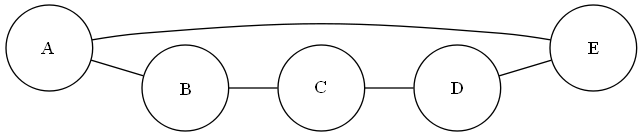
\includegraphics[width=3in]{figures/circle.png}} \\\\
\AnswerOneCiv

\end{tabular}
\end{subquestion}

\vspace{-.15in} 
\begin{subquestion}[2]{}\\
\begin{tabular}{cl}

\multirow{1}{*}{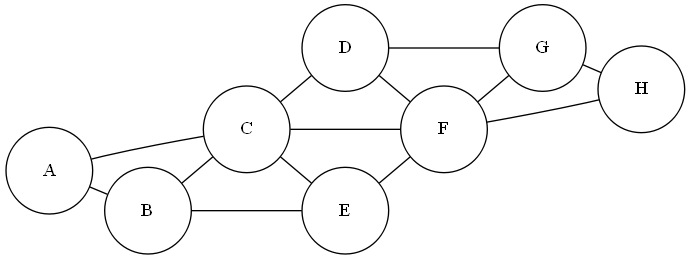
\includegraphics[width=3in]{figures/csp_graph.png}} \\\\
\AnswerOneCv

\end{tabular}
\end{subquestion}



\end{question}